% Preamble
\documentclass[../Relazione_circuiti]{subfiles}
% \usepackage{amstex} Mi si era aggiunto da solo, magari un giorno capiamo che serve

% Packages
\graphicspath{{\subfix{../images/}}}

% Document
\begin{document}

Il filtro crossover è un circuito RLC costituito da due rami: uno con un filtro passa basso realizzato mediante un
induttore e una resistenza in serie (ramo \textbf{Woofer}), l'altro un filtro passa alto realizzato mediante
condensatore e resistenza in serie (ramo \textbf{Tweeter}). Le due resistenze sono identiche a meno dell'incertezza.

\begin{figure}[H]
  \centering
  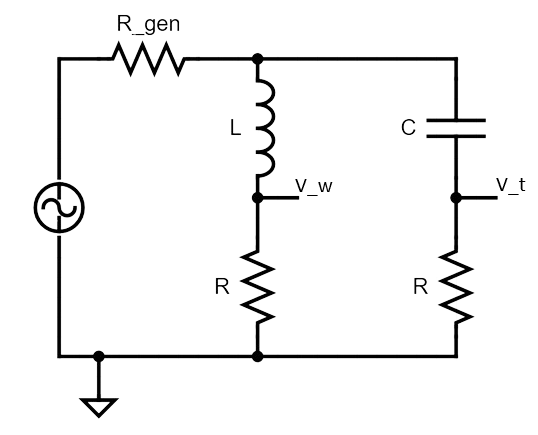
\includegraphics[width=8cm]{Schema_crossover.png}

  \caption{Schema del circuito}
  \label{fig:schema_circuito}

\end{figure}

In risposta ad un segnale oscillante in ingresso, questo è attenuato in ampiezza dal ramo Woofer se a frequenza elevata,
attenuato dal ramo Tweeter se a bassa frequenza. L'attenuazione tuttavia non è nettamente definita nell'intorno di un
valore di frequenza dipendente dalle caratteristiche del circuito. Si definisce frequenza di crossover $f_{cross}$ la
frequenza a cui l'ampiezza dei due segnali è uguale:

\begin{equation}
  \label{eq:f_cross}
  f_{cross} = \frac{1}{2 \pi \sqrt{LC} }
\end{equation}

dove $L$ è l'induttanza della bobina sul ramo Woofer e $C$ la capacità del condensatore sul ramo Tweeter.

Si ha inoltre, sempre alla suddetta frequenza, uno sfasamento dei due rami rispetto al generatore uguale e opposto: il
Woofer anticipa, il Tweeter ritarda.

\begin{align}
  \phi_{woofer} &= \arctan(-\frac{\omega L}{R}) \label{eq:p_woofer} \\
  \phi_{tweeter} &= \arctan(\frac{1}{\omega RC}) \label{eq:p_tweeter}
\end{align}

%\begin{equation} \label{eq:p_woofer}
%  \phi_{woofer} \; = \; \arctan(-\frac{\omega L}{R})
%\end{equation}
%\begin{equation} \label{eq:p_tweeter}
%  \phi_{tweeter} \; = \; \arctan(\frac{1}{\omega RC})
%\end{equation}

dove $L$ e $C$ sono definiti come in \eqref{eq:f_cross}, $\omega$ è la pulsazione dell'onda in ingresso, $R$ la resistenza
(identica su entrambi i rami).

\subsection{Misure effettuate}
  Abbiamo misurato l'ampiezza di entrambi i canali in funzione della frequenza, riferita al ground del circuito.

  La fase invece è stata misurata rispetto al canale Woofer. Si ha quindi che la fase del Tweeter rispetto al Woofer
  rappresenta in realtà la differenza di fase tra i due riferita al generatore.

  \begin{equation}
    \label{eq:p_diff}
    \phi_{diff} \; = \; \arctan(\frac{\omega L}{R}) + \arctan(\frac{1}{\omega RC})
  \end{equation}

  Alla frequenza di cross la differenza di fase vale

  \begin{equation}
    \label{eq:p_diff_cross}
    \phi_{cross} \; = \; 2 \arctan(\frac{1}{R} \sqrt{\frac{L}{C}})
  \end{equation}

\end{document}